\section{\asd Policy}
\label{sec:policy}
In this section, we first present the \asd policy language for controlling app's behavior during its execution. Afterwards, we will present  how to define in \asd policies discussed in our application scenario ( see Section \ref{sec:app-scenario}). Finally, we provide some details on how policies can be automatically generated. 

\subsection{Policy Language}
Figure \ref{fig:lang} shows the the syntax of \asd policy. Policies are identified by a name and they define what \textit{operation} a \textit{Requester} application can execute on a \textit{Resource}. In our prototype we defined two sets of \textit{operations}: the first set contains getter methods that return data from the Resource to the Requester; the second set contains  setter methods where data is being passed by the Requester to the Resource. Moreover, \asd offers the possibility to define policies on events (i.e. boot completed, app installed, app running, etc\ldots). The operations defined in the policies are then mapped to Java methods or native functions that \asd will interpose at runtime to enforce the policies.

\begin{figure}[ht!]
\centering
\lstinputlisting[language=Java]{mysnippets/lang.txt}
\caption{\asd Policy Language}
\label{fig:lang}
\end{figure}

In \asd, a Resource identifies any sensitive data which could be retrieved via either Android middleware API (i.e., location, contact, camera) or native code (i.e., sensors, socket, microphone). 
 
The \textit{have to perform} clause  specifies which actions have to be performed if this policy is enforced. These actions are mappped to a set of functions to control the app's behavior (i.e., filtering, anonymisation, etc.) and to change the values of the parameters of the operation being executed. An action is a callback that is registered by \asd to dynamically forward the execution to the corresponed function and  can operate on both input parameters and returned values. 

A policy can have an optional clause \textit{if} that defines a condition that must be verified before the specified action is performed. Otherwise, if the condition is not true, the action specified in the policy is not executed. 


\subsection{Fine-Grained Access Control Policies}
\label{sec:finepolicy}
We begin with some examples of policies for fine-grained control over apps accessing user data or using network access. Any  access to a protected resource is intercepted by the hooking mechanism and diverted through a custom user-defined control code. \\
As discussed in Section \ref{sec:app-scenario}, the enterprise $Ent$ wants to enforce fine-grained app-level policies. In this scenario, $Ent$ wants to protect business data (i.e., contact and calendar) against unauthorized operations according to custom corporate-level policies and protect the managed app enforcing integrity checks at runtime. Moreover, $Ent$ wants that any connection made by a specific set of apps makes use of a secure channel (i.e., TLS) thus reporting any connection which makes use of insecure transport system like HTTP. The enterprise's requirements can be expressed by policies shown in Figure \ref{fig:policies}. \\

\begin{figure}[ht!]
\centering
\lstinputlisting[language=Java]{mysnippets/policies.txt}
\caption{\asd Policies}
\label{fig:policies}
\end{figure}

\textit{MicPolicy} in Figure \ref{fig:policies}, is quite straightforward: any request for accessing to microphone capabilities made by managed apps is restricted by the policy such that \asd intercepts the request and checks for the specified condition (if clause) , if it is validated then the access is denied. Another similar policy is \textit{LocPolicy}. Such policy permits to avoid location information leak potentially made via apps during working hours. The artificial value returned by \asd is totally controllable by the user, by default \asd returns an existing location chosen at random among a user predefined set of positions.

The policy \textit{ContPolicy}, line 9,  permits to achieve a content provider isolation for an \asd managed app. In this specific case, $Ent$ wants to isolate corporate business contacts sharing them only across authorized apps that have been register throught the \asd Enteprise Policy Manager (see Section \ref{sec:polman}). Moreover, the $Ent$ wants to specify particular criteria that must be respected to allow to the managed app to access business contacts data. In particular, the policy ContPolicy operates as following. The requested operation getContact indicates that any kind of attempt to retrieve the user contacts list must be intercepted and monitored by \asd. Then, for each intercepted operation the specified conditions must be verified. The user-defined isWorkHours() function returns True whether the actual time is within the current working time, False otherwise. If isWorkHours() returns True then the specified action is executed. Otherwise, the execution flow will continue as if \asd was not in place. Thanks to this policy, $Ent$ is allowed to specify a customizable fine-grained access policy enforcing access to the isolated corporate contact provider exclusively to apps managed via \asd.


The policy \textit{HTTPPolicy} (line 13), permits to filter out any connection that is being made via HTTP protocol. Connections instantiate by the managed app can be intercepted and monitored by either hooking the appropriate Java level APIs or intercepting native layer functions if needed. The policy specifies that any operation recognized as an attempt to create a connection has to be intercepted and monitored by \asd. The condition verifies whether the request is made during the working time. In this specific case, $Ent$ wants to deny insecure connections made via HTTP protocol. \\

As an example of a policy defining an artifact Resource, \textit{CopPolicy} is presented. It enables the enterprise to specify a custom integrity check to be enforced before the managed app start its execution. Given a specific app, the enterprise wants to verify that its bytecode has not been tampered with. Here we stress that \asd does not require to modify the app's bytecode, thus its checksum value does not change. Thanks to this policy, before each execution of the managed app \asd
computes the app's bytecode checksum value to guarantee that it has not been tampered with. \\
In the following we present and discuss how \asd policies can be automatically generated by the enterprise.

\subsection{Policy Generation}
In this section we present how \asd policies can be automatically generated by extracting information from the policy specification file. The overall procedure of policy creation is presented by Figure \ref{fig:genpolicy}. The policy generator takes as input the policies specification, the sets of Resource that $Ent$ wants to protect (Res.) and the information about what operation is offered by what Resource (Op.). In our current prototype, we selected sensitive resources (i.e., contacts, location, internet access) and we grouped them by the relative requested permissions. Then we used the information offered by PSCout\cite{au2012pscout} to aggregate Android APIs in terms of which permissions are needed by them. At this point, in our prototype we manually selected which API methods belong to a Getter or Setter operation. By doing this we created a mapping between Resource, Operation and the API methods which are offering capabilities to execute that specified Operation on that specified Resource. It is worth noting that $Ent$ can simply extend those sets including any resource that wants to enforce, as presented for \textit{CopPolicy}.
In Table \ref{tab:map} we reported the mapping was used for the policy HTTPPolicy. For the sake of understanding we included only the Android APIs offering HTTP capabilities as they are suggested by the official Android developer guide\footnote{\url{https://developer.android.com/training/basics/network-ops/index.htm}}. The policy expressed by the specification shown in Figure \ref{fig:policies} line 13, produces according to the requested operation on the specified Resource the interposition of the API methods listed in the third column of Table \ref{tab:map}. \\
Finally, the policy generator produces as output the executable file encoding the corporate app-level policies that will be loaded by \asd to enforce at runtime the policies taken as input by the generator.

\newcolumntype{L}[1]{>{\raggedright\let\newline\\\arraybackslash\hspace{0pt}}m{#1}}
\newcolumntype{C}[1]{>{\centering\let\newline\\\arraybackslash\hspace{0pt}}m{#1}}

\begin{table}[!htbp]
%\begin{minipage}{.5\textwidth}
\caption{HTTP-Policy Generation - Intercepted APIs}
\label{tab:map}
\centering	
\begin{tabular}{@{}cc@{}} \toprule
Operation & API to hook (clsname, mname) \\
\cmidrule(l){1-2}
\multirow{2}{*}{createConnection} & (HttpURLConnection , $<init>$)  \\
 & (URL , $<init>$)  \\
 & (URL , openConnection) \\
\bottomrule
\end{tabular}
\end{table}


\begin{figure}[H]
\centering
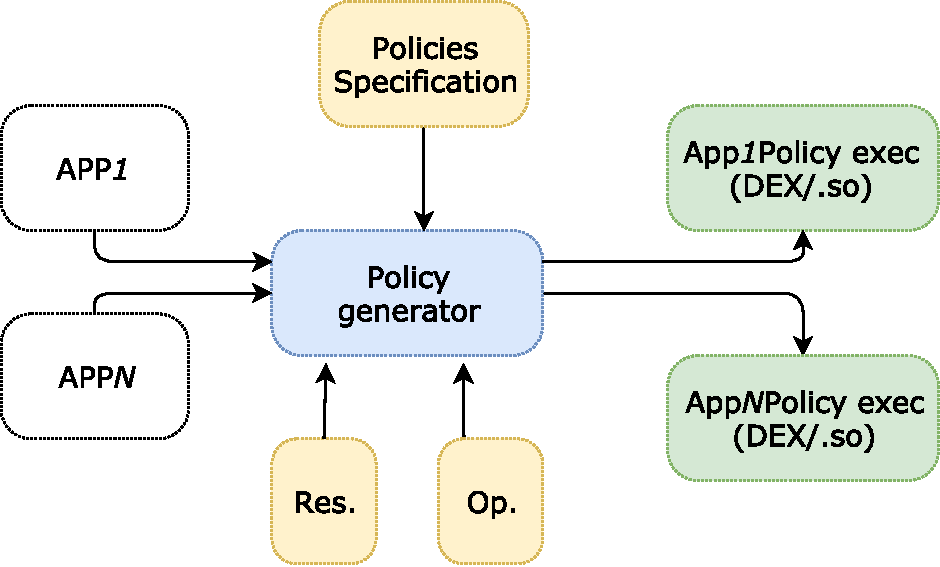
\includegraphics[width=.55\textwidth, keepaspectratio, resolution=600]{policy_gen}
\caption{Policy generation mechanism. Res.: sets of Resource, Op: sets of operation}
\label{fig:genpolicy}
\end{figure}

